\iffalse
\let\negmedspace\undefined
\let\negthickspace\undefined
\documentclass[a4,12pt,onecolumn]{IEEEtran}
\usepackage{amsmath,amssymb,amsfonts,amsthm}
\usepackage{algorithmic}
\usepackage{graphicx}
\usepackage{textcomp}
\usepackage{xcolor}
\usepackage{txfonts}
\usepackage{listings}
\usepackage{enumitem}
\usepackage{mathtools}
\usepackage{gensymb}
\usepackage[breaklinks=true]{hyperref}
\usepackage{tkz-euclide}
\usepackage{listings}
\usepackage{circuitikz}
\usepackage{gvv}
\begin{document}
\title{
\Huge\textbf{ GATE 2023 Assignment}\\
\Huge\textbf{EE1205} Signals and Systems\\
}
\large\author{Kurre Vinay\\EE23BTECH11036}
\maketitle
\textbf{Question:}
In the circuit shown ,$\omega=100\pi\text{rads/s}$, $R_1$=$R_2$=$2.2\Omega$ and $L$=$7\text{mH}$. the capacitance $\text{C}$ for which $Y_{in}$ is purely real is \underline{\hspace{1cm}}  $\text{mF}$ \\
	\begin{center}
	\begin{circuitikz} \centering \draw 
		(0,4) to[sinusoidal voltage source, l=$V_{0}$cos($\omega$t)] (0,0)
		(0,4) to[short] (4,4)
		(4,4) to[resistor, l=$R_1$ ] (4,2)
		(4,2) to[inductor, l= $\text{L} $] (4,0) to[short ] (0,0)
		(8,4)  to[short] (4,4)
		(8,4) to[resistor, l= $R_2$] (8,2) to[capacitor,l=$\text{C}$] (8,0) to (4,0);
	\end{circuitikz}
	\end{center}
\hfill(GATE IN 2023 )\\
\solution\\
\fi
\begin{table}[ht!]
\begin{center}

\begin{tabular}{|c|c|c|c|}
   \hline
   variable&value&description&formulae \\
   \hline
   $Y_{in}$ & -& Admittance of circuit&$\frac{R_1-Ls}{R_1^2-\brak{Ls}^2} + \frac{R_2-\frac{1}{ \text{sC}}}{R_2^2-\brak{\frac{1}{ \text{sC}}}^2}$\\
   \hline
   $X_{L}$ & $7s\Omega$ & Inductive reactance&$\text{sL}$ \\
   \hline
   $X_{C}$ &$\frac{1}{s\text{C}}\Omega $ & Capacitive reactance& $\frac{1}{s\text{C}}$\\
   \hline
    $\text{s}$& $100\pi\text{j}$&Laplace complex frequency&$j\omega$\\
   \hline
   $\omega$ &$100\pi$rads/s& Angular frequency&-\\
   \hline
   $\text{V}$&$V_{0}$cos($\omega$t)&voltage of source&-\\
   \hline
   $R_1 , R_2$& $2.2\Omega$ &resistance of resistors&-\\
   \hline
 
\end{tabular}
\caption{Table: Input Parameters}
\label{tab:1.46Q}
\end{center}
\end{table}
\\From $\tabref{tab:1.46Q}$
\begin{align} 
Y_{in}&=\frac{R_1-Ls}{R_1^2-\brak{Ls}^2} + \frac{R_2-\frac{1}{ \text{sC}}}{R_2^2-\brak{\frac{1}{ \text{sC}}}^2}\\
Im\brak{Y_{in}}&=\frac{-Ls}{R_1^2-\brak{Ls}^2} + \frac{-\frac{1}{ \text{sC}}}{R_2^2-\brak{\frac{1}{ \text{sC}}}^2}
\end{align}
According to the question given, $Y_{in}$ is purely real , so imaginary part should be equal to zero\\
Take the values from $\tabref{tab:1.46Q}$\\
\begin{align}
 \frac{-1}{4.4}+\frac{\frac{1}{ (100\pi) \text{C}}}{(2.2)^2+\brak{\frac{1}{ (100\pi) \text{C}}}^2}&=0\\ 
 \frac{\frac{1}{ (100\pi) \text{C}}}{(2.2)^2+\brak{\frac{1}{ (100\pi) \text{C}}}^2}&=\frac{1}{4.4}\\
  (2.2)^2-\frac{4.4}{ (100\pi) \text{C}}+\brak{\frac{1}{ (100\pi) \text{C}}}^2&=0\\
 \brak{2.2-\frac{1}{ (100\pi) \text{C}}}^2&=0\\
 \frac{1}{ (100\pi) \text{C}}&=2.2\\
 \text{C}&=\frac{700}{484}\text{mF}\\
 \text{C}&=1.446281\text{mF}
\end{align}
The capacitance of capacitor $\text{C}$ is 1.45$\text{mF}$
\begin{figure}[ht!]
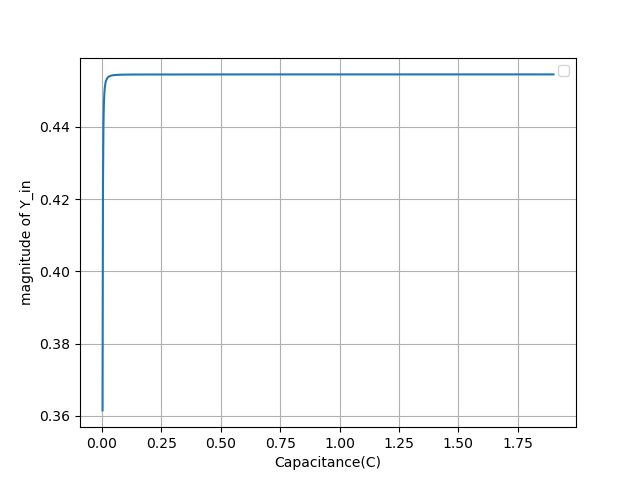
\includegraphics[width=\columnwidth]{figs/fig2.png}
\caption{\large{the plot of capacitance vs magnitude of $Y_{in}$}}
\end{figure}

\end{document}
